\documentclass[letterpaper,11pt]{article}
\usepackage{graphicx}
\usepackage{listings}
\usepackage[super]{nth}
\usepackage[hyphens]{url}
\usepackage{hyperref}
\usepackage{amsmath}
\usepackage[makeroom]{cancel}
\usepackage[table]{xcolor}
\usepackage{comment}
\usepackage[space]{grffile}

\newcommand*{\srcPath}{../src}%

\lstset{
	basicstyle=\footnotesize,
	breaklines=true,
}

\begin{document}

\begin{titlepage}

\begin{center}

\Huge{Assignment 1}

\Large{CS 532:  Introduction to Web Science}

\Large{Spring 2017}

\Large{Grant Atkins}

\Large Finished on \today

\end{center}

\end{titlepage}

\newpage


% =================================
% First question
% =================================
\section*{1}


\subsection*{Question}

\begin{verbatim}
1.  Demonstrate that you know how to use "curl" well enough to
correctly POST data to a form.  Show that the HTML response that
is returned is "correct".  That is, the server should take the
arguments you POSTed and build a response accordingly.  Save the
HTML response to a file and then view that file in a browser and
take a screen shot.
\end{verbatim}

\subsection*{Answer}

The curl command is capable of solving this problem multiple ways. As stated by the Curl manual	 page, curl offers two options to post data:

\begin{itemize}
  \item -F, --form, 'type='
  \item -d, --data, 'type='
\end{itemize}

The difference between the two is the content-type, where -F is multipart/form-data and -d is application/x-www-form-urlencoded \cite{curlref}. Meaning -F can send files and parameters, while -d can just be used to send parameters via HTTP post.

For simplicity, I chose the latter route and used -d as part of my curl commands. I also chose to include -o, --output, which outputs the response to a file. The commands are as follows:

\lstinputlisting[frame=single,caption={Curl with and without post parameters},label=lst:q1fetch,captionpos=b,numbers=left,showspaces=false,showstringspaces=false,basicstyle=\footnotesize]{\srcPath/curlCommand.sh}

The first command sends two parameters in a post request to a URI, more specifically a PHP file that I created in my personal public html directory on the ODU Computer Science servers. The PHP file, as shown below in Listing \ref{lst:q1php}, expects two parameters which are: name and note. Those two parameters are then included inside of the html document response to show they were posted correctly, also the banner in which they are displayed should turn green if posted correctly like shown in Figure \ref{fig:q1correctResponse}. The second command shows a curl command without post parameters to the same URI. This should show a red banner with an insult on your use of curl like shown in Figure \ref{fig:q1incorrectResponse}.

\lstinputlisting[frame=single,caption={PHP Script for receiving form post parameters},label=lst:q1php,captionpos=b,numbers=left,showspaces=false,showstringspaces=false,basicstyle=\footnotesize]{\srcPath/curlPost.php}

\clearpage

\begin{figure}[h]

\includegraphics[scale=0.26]{correctResponse.png}
\caption{Correct response rendered in browser}
\label{fig:q1correctResponse}
\end{figure}

\lstinputlisting[frame=single,caption={Correct response html content outputted by curl command},label=lst:q1fetch,captionpos=b,numbers=left,showspaces=false,showstringspaces=false,basicstyle=\footnotesize]{\srcPath/output/correctResponse.html}

\clearpage

\begin{figure}[h]
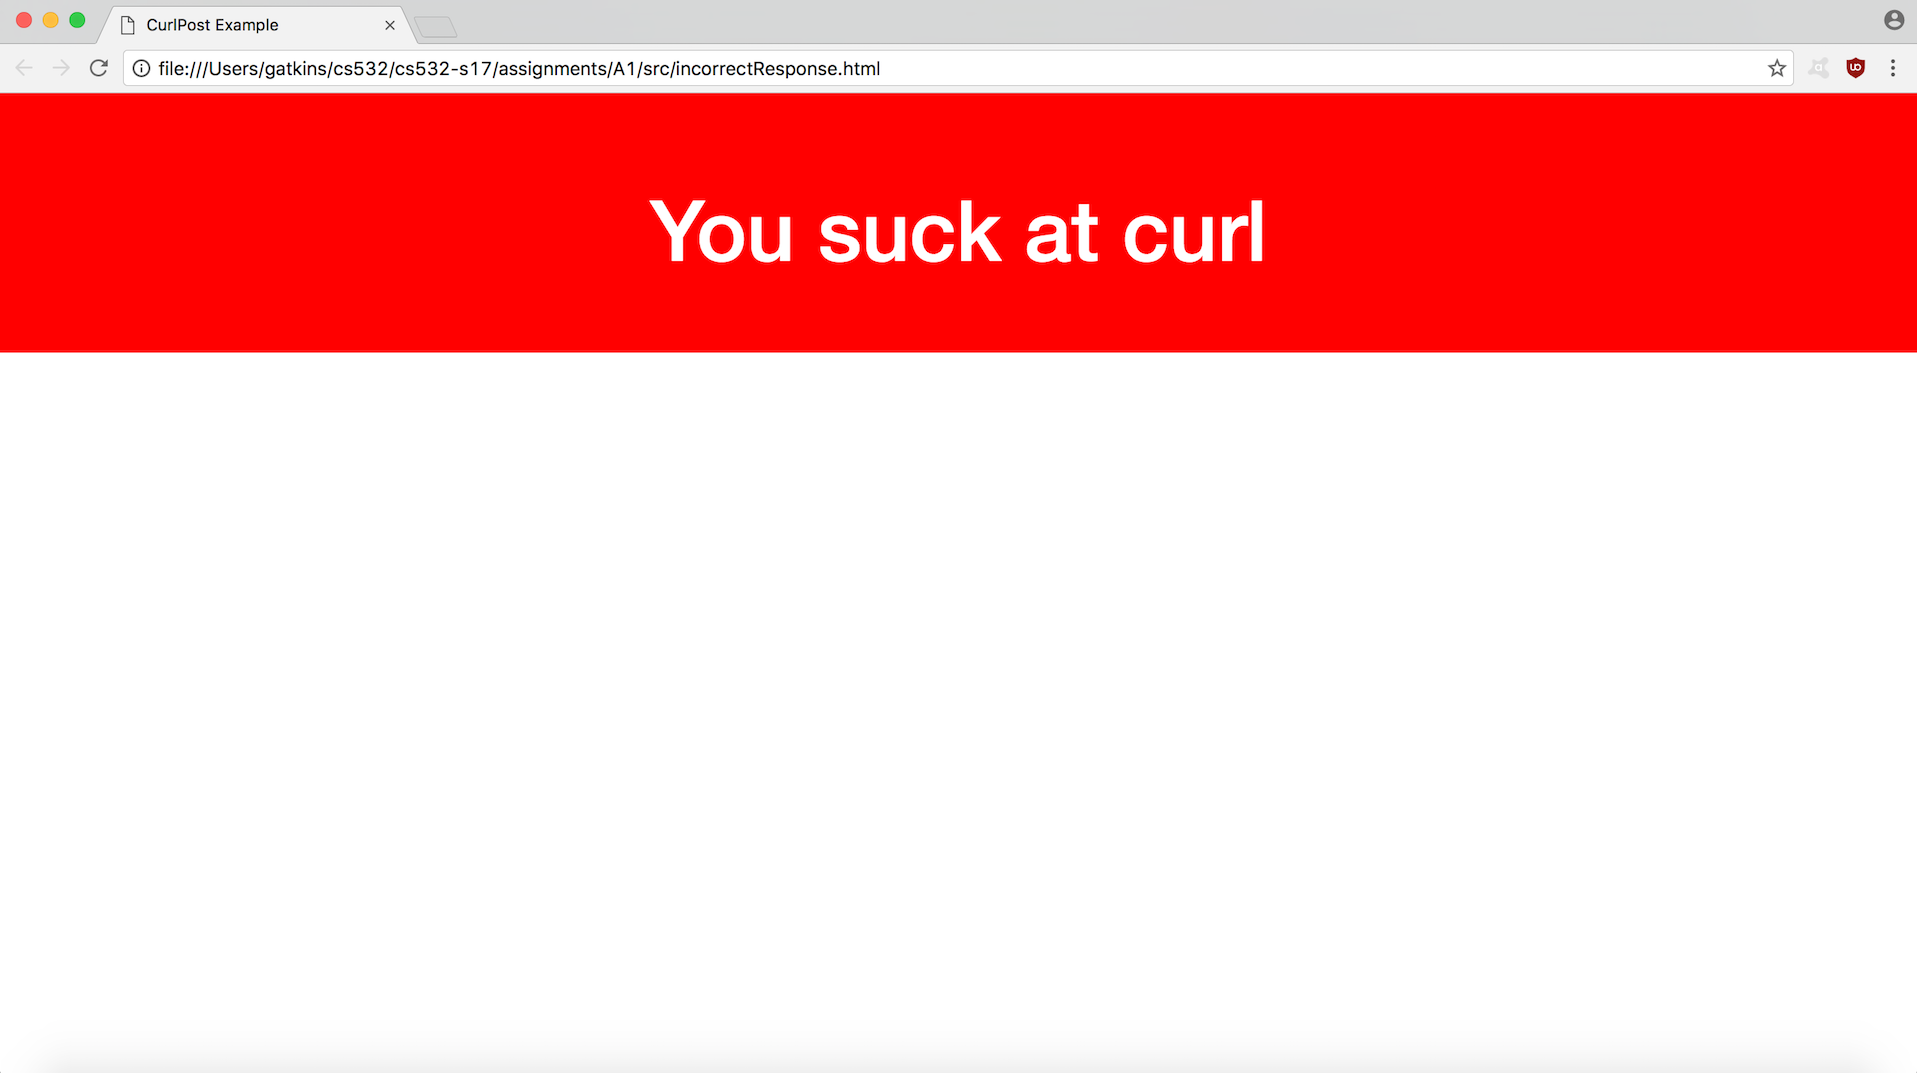
\includegraphics[scale=0.26]{incorrectResponse.png}
\caption{Incorrect response rendered in browser}
\label{fig:q1incorrectResponse}
\end{figure}

\lstinputlisting[frame=single,caption={Incorrect response html content outputted by curl command},label=lst:q1fetch,captionpos=b,numbers=left,showspaces=false,showstringspaces=false,basicstyle=\footnotesize]{\srcPath/output/incorrectResponse.html}

\clearpage

% =================================
% Second question
% =================================

\section*{2}

\subsection*{Question}

\begin{verbatim}
2.  Write a Python program that:
  1. takes as a command line argument a web page
  2. extracts all the links from the page
  3. lists all the links that result in PDF files, and prints out
     the bytes for each of the links.  (note: be sure to follow
     all the redirects until the link terminates with a "200 OK".)
  4. show that the program works on 3 different URIs, one of which
     needs to be: 
     http://www.cs.odu.edu/~mln/teaching/cs532-s17/test/pdfs.html
\end{verbatim}

\subsection*{Answer}

\lstinputlisting[frame=single,caption={Python script that searches for links that end in pdf files},label=lst:q2fetch,captionpos=b,numbers=left,showspaces=false,showstringspaces=false,basicstyle=\footnotesize]{\srcPath/pdfCrawl.py}

This script was written in python, and requires version 2.7 which is currently the default for mac computers and ODU CS department's servers. My solution took an iterative approach doing one URI at a time and waiting for each response until moving onto the next URI found. This program takes advantage of the built in libraries: 

\begin{itemize}
  \item sys
  \item urllib2
  \item urlparse
  \item httplib
\end{itemize}

It also uses the third party library Beautiful Soup to parse html content received using this program.

The script is run like so:
\begin{lstlisting}[frame=single]
python pdfCrawl.py URI
\end{lstlisting}

Once \verb+pdfCrawl.py+ is run it first checks if there is indeed a URI provided via command line arguments. Then it will pass the first argument after the script name to the function \verb+request+, which takes a properly formatted URI and performs an HTTP get request using the urllib2 library. When performing this request, the urllib2 library takes into consideration: infinite loops from 300 responses, incorrect formatted URIs, no response code at all, and 400 response codes for client errors \cite{urllibref}. I also included the use of the httplib library into this function because there were sometimes special errors when the get request could never fulfill a connection to the server. If none of these errors occurred the request function would return the HTTP get response, otherwise it would return nothing.

After the first request was made it would be passed to \verb+findPdfs+ function which would use Beautiful Soup to find all the html \emph{a} elements that contained \emph{href} tags to another URI \cite{beautifulsoupref}. I would then iterate through each of the URIs found on the page and request again each of those URIs to determine if the URI would point to pdf file. If the final URI provided a content-type of $application/pdf$ and a response code of $200$ it was considered a pdf file.

One of the test cases that came up is whether a URI found in the html document was absolute or relative. Using a script provided from a Stackoverflow.com post, I created a function that determined if a string was relative or absolute \cite{abosoluteurlref}. If it was relative, it would be merged with the original final URI provided from command line to create an absolute URI . There was one case, found in Listing \ref{lst:q2URI3}, that actually didn't return content-length, meaning I had to count the bytes from the response's content instead of getting it from the header information. When the \verb+findPdfs+ function ends it returns an array of pdfs that can be used for further use.

The URIs I used for this problem were:
\begin{itemize}
  \item \url{http://www.cs.odu.edu/~mln/teaching/cs532-s17/test/pdfs.html}
  \item \url{http://www.cs.odu.edu/~zeil}
  \item \url{http://www.cs.odu.edu/~nadeem/classes/cs752-S11/}
\end{itemize}

I ran my script and then saved the output to text files, they are as follows:

\lstinputlisting[frame=single,caption={Output from \url{http://www.cs.odu.edu/~mln/teaching/cs532-s17/test/pdfs.html}},label=lst:q2URI1,captionpos=b,numbers=left,showspaces=false,showstringspaces=false,basicstyle=\footnotesize]{\srcPath/output/uri1Links.txt}

\lstinputlisting[frame=single,caption={Output from \url{http://www.cs.odu.edu/~zeil}},label=lst:q2URI2,captionpos=b,numbers=left,showspaces=false,showstringspaces=false,basicstyle=\footnotesize]{\srcPath/output/uri2Links.txt}

\lstinputlisting[frame=single,caption={Output from \url{http://www.cs.odu.edu/~nadeem/classes/cs752-S11/}},label=lst:q2URI3,captionpos=b,numbers=left,showspaces=false,showstringspaces=false,basicstyle=\footnotesize]{\srcPath/output/uri3Links.txt}


\clearpage

% =================================
% Third question
% =================================

\section*{3}

\subsection*{Question}

\begin{verbatim}
3.  Consider the "bow-tie" graph in the Broder et al. paper (fig 9):
    http://www9.org/w9cdrom/160/160.html

    Now consider the following graph:

    A --> B
    B --> C
    C --> D
    C --> A
    C --> G
    E --> F
    G --> C
    G --> H
    I --> H
    I --> K
    L --> D
    M --> A
    M --> N
    N --> D
    O --> A
    P --> G 
    
    For the above graph, give the values for:

    IN: 
    SCC: 
    OUT: 
    Tendrils: 
    Tubes: 
    Disconnected:
\end{verbatim}

\clearpage
\subsection*{Answer}

\begin{figure}[h]
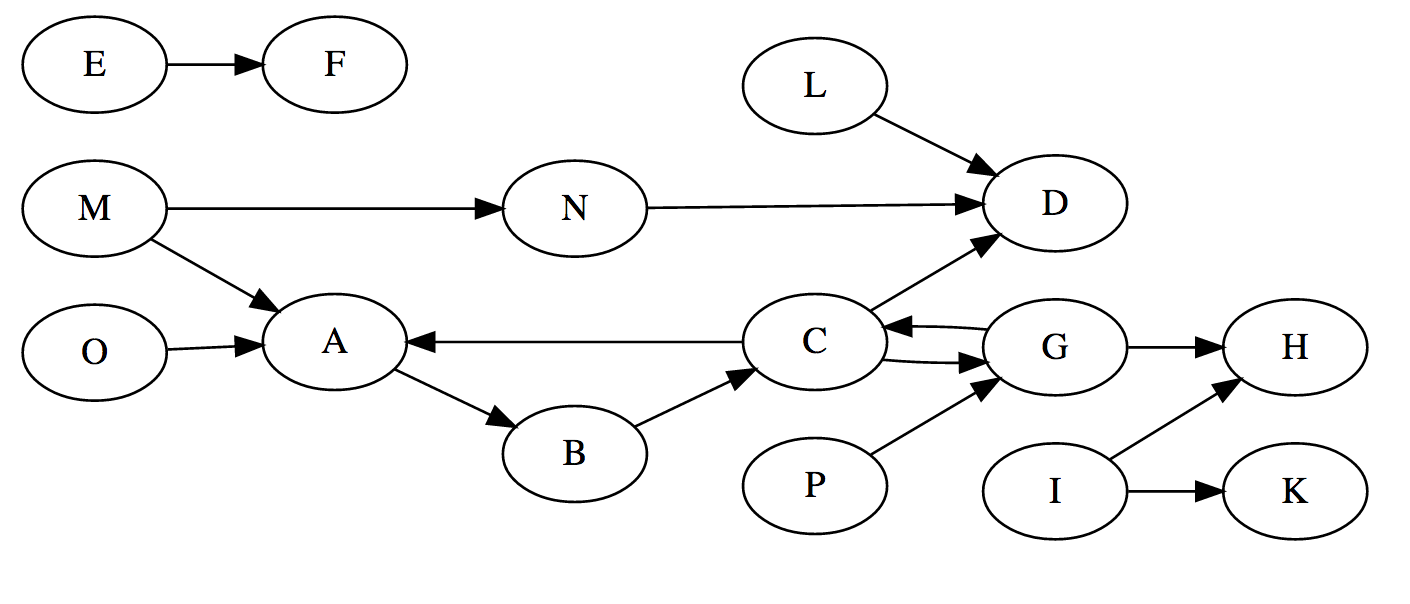
\includegraphics[scale=0.5]{webvizgraph.png}
\caption{Graph representation generated with WebGraphviz \cite{webgraphvizref}}
\label{fig:q3graph}
\end{figure}

\textbf{IN:} M, O, P

These values are considered the \emph{IN} values due to the fact that they can reach values that are considered to be in the \emph{SCC} and also because they can't be reached from the \emph{SCC} \cite{graphstructureref}.	

\textbf{SCC:} A, B, C, G

These values are considered the \emph{SCC} values because they are at the ``heart of the graph.'' They either are all nodes that can reach another node along directed links. This can consist of links from the outside in, nodes inside the \emph{SCC} pointing to other nodes inside, or nodes point from the inside out \cite{graphstructureref}.

\textbf{OUT:} D, H

These values are part of the \emph{OUT} because they are accessible from the \emph{SCC} but they cannot link back into it \cite{graphstructureref}.

\textbf{Tendrils:} I, K, L

These values don't reference the \emph{SCC} at any point, but do have links to the \emph{OUT} nodes and therefore they are considered the \emph{tendrils} \cite{graphstructureref}.

\textbf{Tubes:} N

This value isn't part of the ``heart of the graph'' but it does connect an \emph{IN} node to an \emph{OUT} node in one step, not touching the \emph{SCC} in the process \cite{graphstructureref}.

\textbf{Disconnected:} E, F

These two values are as their title describes - disconnected. They aren't part of the \emph{SCC} and don't connect to anything else on the graph.

\clearpage


\clearpage

% =================================
% Bibliography
% =================================

\begin{thebibliography}{9}
\bibitem{urllibref} 
"20.6. Urllib2 - Extensible Library for Opening URLs." 20.6. Urllib2 - Extensible Library for Opening URLs - Python 2.7.13 Documentation. Python Software Foundation, n.d. Web. 24 Jan. 2017. \url{https://docs.python.org/2/library/urllib2.html}. 
\bibitem{beautifulsoupref} 
Richardson, Leonard. "Beautiful Soup Documentation." Beautiful Soup Documentation - Beautiful Soup 4.4.0 Documentation. N.p., n.d. Web. 24 Jan. 2017. \url{https://www.crummy.com/software/BeautifulSoup/bs4/doc/}.
\bibitem{curlref} 
Stenberg, Daniel. "Curl.1 the Man Page." Curl - How To Use. N.p., n.d. Web. 24 Jan. 2017. \url{https://curl.haxx.se/docs/manpage.html}.
\bibitem{graphstructureref} 
Broder, Andrei, Ravi Kumar, Farzin Maghoul, Prabhakar Raghavan, Sridhar Rajagopalan, Raymie Stata, Andrew Tomkins, and Janet Wiener. "Graph Structure in the Web." 9th International World Wide Web Conference, June 2000. Web. 24 Jan. 2017. \url{http://www9.org/w9cdrom/160/160.html}.
\bibitem{abosoluteurlref} 
Lalinsk�, Luk�. "How Can I Check If a URL Is Absolute Using Python?" Stack Overflow. N.p., n.d. Web. 24 Jan. 2017. \url{http://stackoverflow.com/questions/8357098/how-can-i-check-if-a-url-is-absolute-using-python}.
\bibitem{webgraphvizref} 
"Webgraphviz." Webgraphviz. N.p., n.d. Web. 24 Jan. 2017. \url{http://www.webgraphviz.com/}.
\end{thebibliography}

\end{document}